\documentclass[conference,letterpaper]{IEEEtran}
% Four technical pages and a reference-only fifth page. No margin/font shrinking.
\usepackage[T1]{fontenc}
\usepackage{newtxtext,newtxmath}
\usepackage{amsmath,booktabs,array,tabularx}
\usepackage{graphicx,tikz}
\usetikzlibrary{arrows.meta,positioning,calc}
\usepackage{cite}
\usepackage[hidelinks]{hyperref}
\usepackage{microtype}
\newcommand{\epl}{EP-L2}
\newcommand{\base}{B16}
\newcommand{\unif}{U-WB16}
\newcolumntype{L}[1]{>{\raggedright\arraybackslash}p{#1}}
% Real, fixed-height layout reservations. They intentionally contain no fake data.
\newcommand{\resultpanel}[4]{\fbox{\begin{minipage}[c][#2][c]{\dimexpr#1-2\fboxsep-2\fboxrule\relax}\centering
\small\textbf{#3}\par\medskip
\footnotesize MEASUREMENTS PENDING\par\medskip
\parbox{.91\linewidth}{\centering\footnotesize #4}
\end{minipage}}}
\hypersetup{pdftitle={EP-L2: Elastic Payload Storage for In-Place Writeback in GPU L2 Caches},pdfauthor={EP-L2 project; author information pending},pdfsubject={EN-v5: bounded writeback claims, explicit validation gap, and reserved result panels}}
\hyphenation{write-back micro-ar-chi-tec-ture in-di-rec-tion}
\begin{document}
\title{EP-L2: Elastic Payload Storage for\\In-Place Writeback in GPU L2 Caches}
\author{\IEEEauthorblockN{Author information to be completed}\IEEEauthorblockA{English working draft EN-v5 (SAD intake r1) --- not for submission}}
\maketitle
\begin{abstract}
A fixed-partition L2 may copy a dirty victim into a writeback buffer even though its data do not change. Elastic Payload L2 (EP-L2) retains the victim in its original slot and assigns a different, bank-compatible slot to the incoming resident. The protocol separates resident-tag visibility, payload ownership, and writeback ordering, allowing each resource to retire at its own completion event. Against the specified reference, EP-L2 retains the same payload capacity, bank-service budget, and request-tracking limits while removing resident-to-writeback copying and permitting resident/WB cross-role allocation. Its evaluation separates internal data movement, staging-capacity pressure, and application performance, with equal-capacity static controls needed to identify the value of elasticity. An initial independently accepted SAD control shows nearly unchanged execution time while eliminating measured staging copies. Evidence is limited to the qualified native nonatomic scope; broader performance conclusions and physical PPA benefits remain unestablished.
\end{abstract}
\begin{IEEEkeywords}
GPU, L2 cache, writeback, tag--data decoupling, resource sharing
\end{IEEEkeywords}

\section{Introduction}
A dirty eviction changes which transaction consumes a cache line, but need not change where its data are stored. In the fixed-partition L2 studied here, however, the victim is copied from resident storage to a writeback buffer (WBUF) before its resident slot is reused. A source-bank read and destination-bank write perform the copy; a further read sends the writeback. These operations share modeled bank service with demand accesses and fills.

The copy creates internal traffic, while a fixed WBUF quota can block evictions despite idle slots elsewhere. A larger static WBUF can relieve the quota limit but retains the copy. Avoiding relocation can save service, but improves execution only when that service contributes to progress rather than shifting pressure to another resource.

\epl{} transfers payload ownership instead of location. The dirty data remain in place, and the incoming resident receives another eligible slot. The old tag, local data slot, and writeback-ordering entry retire separately. Resident lookup capacity stays fixed.

Tag--data indirection and storage sharing are established ideas: V-Way decouples placement~\cite{vway}, GPU-local storage can be repartitioned~\cite{unified}, and in-cache MSHRs and MiCache reuse storage for outstanding requests~\cite{farkas,micache}. Our proposed contribution is an \emph{in-place dirty-writeback protocol} with explicit ownership and release obligations, evaluated under a fixed payload and bank-service budget. Its central question is whether copy removal and cross-role allocation improve useful service enough to justify their control cost.

The primary study compares resident/WB pooling with the declared static reference. Concurrent dynamic bypass service and optional victim-retention/read-only extensions are outside that comparison. Strong static controls are needed to distinguish the value of elasticity from the effects of the selected reference partition.

\section{EP-L2 Design}
\subsection{One-Slice Organization and Comparison Boundary}
The primary reference, \base{} (\texttt{B16\_BANKED}), partitions 1168 line-sized slots into 1024 resident, 128 bypass-return, and 16 WBUF slots. \unif{} (\texttt{U\_WB16}) permits resident and WB allocations across this physical pool. Each slot is 128 B with four 32-B sectors. Both modes provision four banks of 292 slots, at most one modeled line-sized operation per bank per physical GPU cycle, and a common 128-B copy latch outside the pool. Both also retain 128 writeback address-directory (WAD) entries and the same request-metadata limits. Sixteen is the static \emph{data} quota, not the U-WB control limit.

\begin{figure*}[t]
\centering
\begin{minipage}[t]{.49\textwidth}
\centering\small\textbf{(a) Logical organization of one L2 slice}\par\smallskip
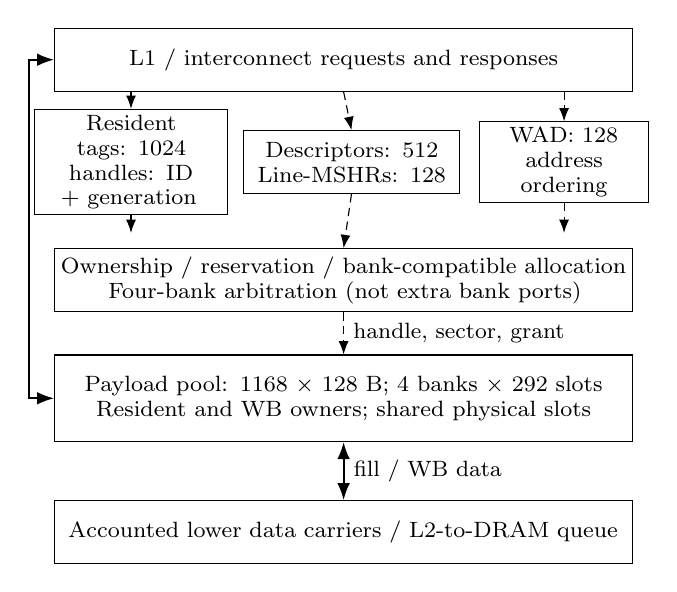
\begin{tikzpicture}[x=1mm,y=1mm,>=Latex,font=\fontsize{8}{9}\selectfont,
box/.style={draw,align=center,inner sep=2pt,minimum height=8mm},
ctl/.style={->,densely dashed,line width=.4pt},data/.style={<->,line width=.7pt}]
\node[box,text width=72mm] (in) at (40,53) {L1 / interconnect requests and responses};
\node[box,text width=23mm] (tag) at (13,40) {Resident tags: 1024\\handles: ID + generation};
\node[box,text width=26mm] (req) at (41,40) {Descriptors: 512\\Line-MSHRs: 128};
\node[box,text width=20mm] (wad) at (68,40) {WAD: 128\\address ordering};
\node[box,text width=72mm] (ctrl) at (40,25) {Ownership / reservation / bank-compatible allocation\\Four-bank arbitration (not extra bank ports)};
\node[box,text width=72mm,minimum height=11mm] (pool) at (40,10) {Payload pool: 1168 $\times$ 128 B; 4 banks $\times$ 292 slots\\Resident and WB owners; shared physical slots};
\node[box,text width=72mm] (low) at (40,-7) {Accounted lower data carriers / L2-to-DRAM queue};
\draw[ctl] (in.south)--(req.north);
\draw[ctl] (13,49)--(tag.north);\draw[ctl] (68,49)--(wad.north);
\draw[ctl] (tag.south)--(13,31);\draw[ctl] (req.south)--(ctrl.north);\draw[ctl] (wad.south)--(68,31);
\draw[ctl] (ctrl.south)--node[right]{handle, sector, grant} (pool.north);
\draw[data] (pool.south)--node[right]{fill / WB data} (low.north);
\draw[data] (in.west)--(0,53)--(0,10)--(pool.west);

\end{tikzpicture}
\end{minipage}\hfill
\begin{minipage}[t]{.49\textwidth}
\centering\small\textbf{(b) Copy removal and separate release events}\par\smallskip
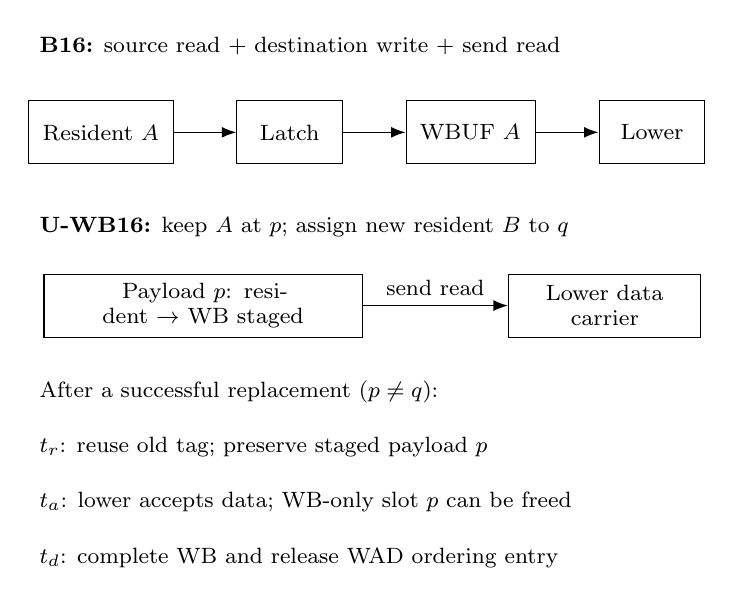
\begin{tikzpicture}[x=1mm,y=1mm,>=Latex,font=\fontsize{8}{9}\selectfont,
box/.style={draw,align=center,inner sep=2pt,minimum height=8mm},arr/.style={->,line width=.5pt}]
\node[anchor=west] at (0,55) {\textbf{B16:} source read $+$ destination write $+$ send read};
\node[box,text width=17mm] (a) at (9,44) {Resident $A$};
\node[box,text width=12mm] (l) at (33,44) {Latch};
\node[box,text width=15mm] (w) at (56,44) {WBUF $A$};
\node[box,text width=12mm] (d) at (79,44) {Lower};
\draw[arr] (a)--(l);\draw[arr] (l)--(w);\draw[arr] (w)--(d);
\node[anchor=west] at (0,32) {\textbf{U-WB16:} keep $A$ at $p$; assign new resident $B$ to $q$};
\node[box,text width=39mm] (p) at (22,22) {Payload $p$: resident $\to$ WB staged};
\node[box,text width=23mm] (lo) at (73,22) {Lower data carrier};
\draw[arr] (p)--node[above]{send read} (lo);
\node[anchor=west] at (0,11) {After a successful replacement ($p\ne q$):};
\node[anchor=west] at (0,4) {$t_r$: reuse old tag; preserve staged payload $p$};
\node[anchor=west] at (0,-3) {$t_a$: lower accepts data; WB-only slot $p$ can be freed};
\node[anchor=west] at (0,-10) {$t_d$: complete WB and release WAD ordering entry};
\end{tikzpicture}
\end{minipage}
\caption{Declared WB-only design, not a physical floorplan or a measured cycle schedule. Dashed links denote control dependencies; solid links denote data movement. B16 uses fixed 1024/128/16 role quotas over the same banks; U-WB16 allows resident/WB allocation across those slots. Concurrent dynamic bypass service is not established. Both retain a 128-B copy latch outside the pool. Optional TVD/RO consumers are not drawn as extra data arrays.}
\label{fig:organization}
\end{figure*}


Figure~\ref{fig:organization} shows the declared service model. WB-only pooling can borrow reference bypass-return slots, but concurrent dynamic bypass use is unvalidated. Idle bypass capacity therefore makes a WB-heavy static control important.

A resident tag names a payload through a slot identifier and generation. Each slot has one authoritative owner; ready/pending sector masks and pins track its consumers. The initial design preserves the resident bank class:
\begin{equation}
 \operatorname{bank}(p)=p\bmod4=\operatorname{tag\_index}\bmod4.
\label{eq:bank}
\end{equation}
A globally free slot is therefore not necessarily a legal landing for a given tag. The 1024 tags bound resident visibility; a temporarily reserved incoming landing is not an additional visible resident line.

\subsection{Replacement as a Transaction}
Before a dirty replacement commits, the controller obtains the address-ordering entry, required issue resources, and a legal landing. In B16, it reads the victim into the latch and writes WBUF before reusing the resident slot. In U-WB16, dirty line $A$ remains in payload $p$ as \texttt{WB\_STAGED}; new resident $B$ receives $q\ne p$. The send read and lower data carrier remain necessary in both modes.

Precheck refusals acquire no visible ownership; bank retries may retain reservations across cycles. The reserved victim, requester, and eventual native tag commit must agree. If an intervening fill changes a subsequent victim selection, the controller must preserve the original transaction or fully roll it back before preparing another. Rollback releases reservations, not bank work already performed.

The repaired release passes producer and independent directed qualification, including the tested cross-cycle boundary. Application qualification remains bounded by the native nonatomic scope below.

\subsection{Separate Release Events}
At committed replacement time $t_r$, the old tag can be reused. Payload $p$ remains protected until actual downstream data acceptance $t_a$. The WAD retains same-address ordering until writeback completion $t_d$. A software queue pointer alone does not constitute a data handoff: a separately accounted lower carrier must own the dirty data before local staging is released. A late event for $A$ uses its own handle/transaction identity, not the tag now naming $B$.

For tracked reads, requester descriptors and payload pins remain live until response-queue acceptance or internal consumption. Line-MSHR retirement and pending-sector completion are checked separately. Neither event releases a WB address-ordering obligation. A read of one ready sector does not imply that an entire line is ready. Atomic and ordinary requests sharing a line additionally require sector-appropriate dirty and version handling.

Local drain progress requires both eventual lower service and a bank retry that remains identifiable until completion or explicit cancellation. An oldest-selected grant alone cannot guarantee progress if its requester changes identity or stops retrying. Whole-GPU deadlock freedom is not established by these local requirements.

\begin{figure*}[t]
\centering
\resultpanel{.486\textwidth}{40mm}{(a) Matched application performance}{Five fixed development workloads.\\Paired cycles and $C_B/C_U$; retain slowdowns.}
\hfill
\resultpanel{.486\textwidth}{40mm}{(b) Observed copy and writeback work}{Completed copy transfers, successful send reads, and actual WB totals.\\Logical classes remain separate.}
\caption{Main-result reservation; no measurements are plotted. Both panels require the same accepted source/binary and matched input scope.}
\label{fig:mainresults}
\end{figure*}


\subsection{Implementation Cost and Separate Extensions}
Primary payload storage is 146 KiB/slice, or 9.125 MiB over 64 slices; common latches add 8 KiB/chip. A slot index requires $P=11$ bits. Explicit tag handles occupy $1024(P+G)$ bits for generation width $G$; up to 128 WB handles require $128(P+G)$ bits plus state and transaction binding. These are gross representations, not measured incremental area: the reference already includes some common fields.

The incremental hardware comparison must account for handle selection, owner/generation checks, bank-compatible allocation, arbitration, and rollback state. Queue depths, generation/pin bounds, pipeline stages, SRAM ports, and the data carrier after $t_a$ need concrete mappings. Symbolic verification versions are not payload RAM. Equal data capacity and bank throughput do not prove equal hit latency, area, clock frequency, or energy. No RTL synthesis or timing/power result is available in this draft.

TVD retains displaced payloads using a shared 128-entry WAD/TVD budget; RO independently controls pending-tag detachment and Line-MSHR bypass under a whole-commandlist read-only oracle. Both remain separate source candidates with validation pending and are OFF in the primary comparison. Neither receives another data/descriptor pool; lookup, retention, and traffic costs require separate evaluation.

\section{Evaluation Methodology}
\subsection{Matched Inputs and Declared Machine}
We use the Accel-Sim SASS flow and GPGPU-Sim performance-model lineage~\cite{accelsim,gpgpusim}. Their published validation does not validate this modified L2. B16 and U-WB16 must execute with the same independently qualified binary, complete trace input, non-mode settings, timing scope, and termination rules. Table~\ref{tab:configuration} records the current ordered research configuration, including the modified L2; it is not a reconstruction of undocumented commercial-cache internals.

\begin{table}[t]
\caption{Declared matched configuration. L2 capacities are per slice.}
\label{tab:configuration}\centering\footnotesize
\begin{tabularx}{\columnwidth}{@{}L{.42\columnwidth}X@{}}
\toprule
Resource & Setting \\
\midrule
Compute / clock domains & 80 SMs; core/ICNT/L2: 1132 MHz; DRAM: 850 MHz \\
L1 (fixed) & 64 KiB/SM; 4 banks; 20-cycle setting \\
L2 tags / data & 1024 tags; 1168 slots, 146 KiB \\
Line / sectors / banks & 128 B / $4\times32$ B / $4\times292$ slots \\
Service / common latch & 1 op/bank/physical cycle / 128 B \\
Descriptors / Line-MSHRs & 512 / 128; 32 requesters/address \\
WAD / lower queue & 128 / 128 entries \\
Chip / memory channels & 64 slices / 32 channels \\
L2 ROP delay & 160-cycle model setting \\
DRAM scheduler / return & 128 / 192 entries per channel \\
WBUF8 sensitivity & 1160 slots, 145 KiB; $4\times290$ slots \\
\bottomrule
\end{tabularx}
\end{table}

The fixed development set contains convolutionSeparable, FWT\_7\_21, cfd\_097k, vectorAdd\_4M, and sad. Their input sizes and complete commandlists must be bound to the accepted trace manifests; names alone do not specify reproducible experiments. Sad is the predeclared negative control, not a verified low-pressure result. Btree and dwt2d are held out until policy selection; scan is a separate long-running case. These choices do not establish coverage of GPU workloads in general. All five development pairs, including slowdowns, are required before reporting their geometric mean.

\subsection{Correctness Before Performance}
The repaired producer and its independent replay each pass 31 directed invocations, and Lane5 accepts the complete eleven-gate protocol. Per-spec complete-content proofs restrict application qualification to native nonatomic inputs. New results remain bound to the exact source, binary, configurations, and input content.

Required cases cover host-prefill identity and refusal, physical-cycle bank grants, generation reuse, partial/out-of-order sectors, response backpressure, and distinct WB acceptance/completion events. Native tag timestamps may include a host-copy ordering offset; this offset must not supply additional bank-service cycles. Atomic/ordinary sector mixtures need dedicated validation rather than being inferred from ordinary-read/write tests.

SASS traces do not supply complete numerical payloads. The supported checks concern ownership, symbolic sector versions, requester/transaction identity, and resource drain; they are not full numerical application verification. A historical passing run cannot override a later withdrawal of its producing implementation.

\section{Results and Causal Analysis}
\noindent\textbf{Current evidence.} Lane5 ledger generation 8 accepts 5/5 prescribed pairs; this revision independently ingests only SAD (1/5). SAD takes 110,773/110,749 cycles for B16/U-WB16, with 3,975/0 copy transfers and 483,611/475,661 logical bank operations. Both report zero WB-data-full events. The 24-cycle difference is a near tie; the operation reduction is consistent with copy removal, without establishing capacity benefit or behavior of other applications. No group mean or physical PPA result is reported. Figures~\ref{fig:mainresults}--\ref{fig:controls} retain their reservations for later consolidated results.

\subsection{Performance and Internal Movement}
Figure~\ref{fig:mainresults}(a) compares full-run cycles using $S=C_{\base}/C_{\unif}$, with matching instruction counts and timing scope. The geometric mean is defined only over the complete five-pair set. Absolute paired cycles and failures remain available with the results.

For one committed, non-rolled-back WB episode in the declared model, B16 uses two copy operations and one send read; U-WB uses the send read. This is an operation count, not a predicted speedup. Figure~\ref{fig:mainresults}(b) therefore retains actual WB totals, completed copy transfers, and successful send reads. Different eviction counts, retry attempts, and work before rollback must not be hidden by multiplying one mode's WB count by a fixed saving. Existing logical classes combine some copy and demand operations; an exact physical decomposition requires additional audited event attribution.

\begin{figure*}[t]
\centering
\resultpanel{.319\textwidth}{43mm}{(a) Capacity and ordering}{WB-data pressure; staged/reserved slots; eligible-landing failures.\\WAD pressure separately.}
\hfill
\resultpanel{.319\textwidth}{43mm}{(b) Bank work and service}{Logical operations; successful physical grants; per-operation waiting.\\One operation/bank/physical cycle.}
\hfill
\resultpanel{.319\textwidth}{43mm}{(c) Downstream effects}{Matched lower/DRAM traffic and queue pressure.\\Separate data acceptance from WB completion.}
\caption{Causal-analysis reservation. Consistent scopes, denominators, and units are required; a lower counter alone does not establish useful progress.}
\label{fig:causal}
\end{figure*}


\subsection{Pressure, Useful Service, and Ordering}
A borrowing counter is not evidence of a capacity bottleneck. Figure~\ref{fig:causal}(a) requires the static WB-data-full events, staged/reserved occupancy, and candidate pool/eligible-landing failures. WAD-full pressure is separate because the data pool does not enlarge the address directory. Tag-visible residents, temporary landings, and global pool-free slots must also be distinguished: subtracting all resident-role reservations from a 1024-tag limit is not a valid free-capacity measure.

Figure~\ref{fig:causal}(b) separates logical work, physical grants, and waiting; summed operation waits are not elapsed GPU cycles. Figure~\ref{fig:causal}(c) tests pressure transferred to lower queues or DRAM. All panels require common application-cumulative scopes and explicit units. Overlapping intervals are not summed, and missing counters are not zero-filled.

\begin{figure}[t]
\centering
\resultpanel{\columnwidth}{32mm}{Equal-capacity static control}{Primary control: same total slots, different fixed role quotas.\\WBUF8 sensitivity is a separate experiment, not a substitute.}
\caption{Control reservation. Implemented and qualified fixed-total controls are needed before claiming a benefit of elasticity beyond the selected static split.}
\label{fig:controls}
\end{figure}


\subsection{What the Controls Must Establish}
B16 versus U-WB16 tests the combined effect of copy removal and cross-role allocation against one fixed split. It does not isolate either effect. This distinction is especially important when the reference's bypass partition is idle: a WB-heavy static split may remove the apparent capacity shortage without a dynamic allocator.

An equal-1168-slot static control is therefore required before attributing an advantage to elasticity beyond that split. The previously proposed 1024/112/32 partition is an informative comparison, not proof of the best static allocation. It is not yet executable in the frozen 8/16-WBUF interface. A valid control needs explicit quota support, unchanged bank/control resources, and independent qualification. Merely setting WBUF32 would change the physical budget rather than provide the intended comparison.

WBUF8 uses a different matched total of 1160 slots. It measures budget sensitivity, not the missing fixed-total control. Likewise, an ideal diagnostic is not a realizable competitor. If equal-capacity controls remain unavailable, the result must be limited to the specified B16 comparison; independent copy and capacity benefits cannot be claimed.

When local service improves without application benefit, a representative baseline/mechanism $\times$ original/justified downstream-headroom comparison can test the interaction. Ideal WB, metadata, and read-hit cases require their own qualified, same-binary baseline. Such analyses should answer an observed ambiguity, not expand the experiment set without a question. Additional hit/control latency and implementation cost must also be assessed before making efficiency claims; fewer bank operations alone do not establish energy savings.

\section{Related Work and Scope}
\textbf{Flexible placement and shared storage.} V-Way uses additional tags and indirection for demand-based associativity~\cite{vway}; Tag-Split Cache changes data-storage granularity while retaining coarse requests~\cite{tsc}. \epl{} holds resident tags and line/sector sizes fixed. Gebhart \emph{et al.} repartition SM-local register, cache, and scratchpad resources at kernel boundaries; their evaluated cache is write-through~\cite{unified}. 

\textbf{Transient state and miss handling.} In-cache MSHRs reuse cache storage for pending-load information~\cite{farkas}. MiCache shares FPGA storage between cache lines and MSHR subentries, converting pending-request entries into cache entries on response~\cite{micache}. DL-MSHR adapts linked primary/secondary-miss slots, which can also carry write-miss data~\cite{dlmshr}. The proposed distinction is retaining existing dirty data at the same physical location while tag visibility and writeback ordering retire separately. The comparison concerns data lifetime rather than miss-tracker organization.

MRPB reorders and bypasses GPU L1 requests~\cite{mrpb}, while victim caching retains displaced lines for reuse~\cite{victim}. TVD/RO combinations require separate evaluation; additive benefit is not assumed.

\section{Conclusion}
\epl{} proposes to keep dirty data in place when their owner changes from a resident line to a writeback transaction. The protocol separates tag visibility, payload storage, and address ordering under a fixed data and bank-service budget. Its value depends on correct multi-cycle ownership, actual copy/staging pressure, and the cost of the added control. Matched application results and strong static controls remain necessary to establish that value.

% Keep the optional fifth page reference-only. No technical appendix on that page.
\clearpage
% Generated by IEEEtran.bst, version: 1.14 (2015/08/26)
\begin{thebibliography}{10}
\providecommand{\url}[1]{#1}
\csname url@samestyle\endcsname
\providecommand{\newblock}{\relax}
\providecommand{\bibinfo}[2]{#2}
\providecommand{\BIBentrySTDinterwordspacing}{\spaceskip=0pt\relax}
\providecommand{\BIBentryALTinterwordstretchfactor}{4}
\providecommand{\BIBentryALTinterwordspacing}{\spaceskip=\fontdimen2\font plus
\BIBentryALTinterwordstretchfactor\fontdimen3\font minus
  \fontdimen4\font\relax}
\providecommand{\BIBforeignlanguage}[2]{{%
\expandafter\ifx\csname l@#1\endcsname\relax
\typeout{** WARNING: IEEEtran.bst: No hyphenation pattern has been}%
\typeout{** loaded for the language `#1'. Using the pattern for}%
\typeout{** the default language instead.}%
\else
\language=\csname l@#1\endcsname
\fi
#2}}
\providecommand{\BIBdecl}{\relax}
\BIBdecl

\bibitem{vway}
M.~K. Qureshi, D.~Thompson, and Y.~N. Patt, ``The {V-Way} cache: Demand-based
  associativity via global replacement,'' in \emph{Proceedings of the 32nd
  Annual International Symposium on Computer Architecture (ISCA)}, 2005, pp.
  544--555.

\bibitem{unified}
M.~Gebhart, S.~W. Keckler, B.~Khailany, R.~Krashinsky, and W.~J. Dally,
  ``Unifying primary cache, scratch, and register file memories in a throughput
  processor,'' in \emph{Proceedings of the 45th Annual IEEE/ACM International
  Symposium on Microarchitecture (MICRO)}, 2012, pp. 96--106.

\bibitem{farkas}
K.~I. Farkas and N.~P. Jouppi, ``Complexity/performance tradeoffs with
  non-blocking loads,'' Digital Equipment Corporation, Western Research
  Laboratory, Research Report 94/3, Mar. 1994.

\bibitem{micache}
S.~Xu, S.~Lu, Z.~Shao, X.~Liao, and H.~Jin, ``{MiCache}: An {MSHR}-inclusive
  non-blocking cache design for {FPGAs},'' in \emph{Proceedings of the 2024
  ACM/SIGDA International Symposium on Field Programmable Gate Arrays (FPGA)},
  2024, pp. 22--32.

\bibitem{accelsim}
M.~Khairy, Z.~Shen, T.~M. Aamodt, and T.~G. Rogers, ``{Accel-Sim}: An
  extensible simulation framework for validated {GPU} modeling,'' in
  \emph{Proceedings of the 47th Annual International Symposium on Computer
  Architecture (ISCA)}, 2020, pp. 473--486.

\bibitem{gpgpusim}
A.~Bakhoda, G.~L. Yuan, W.~W.~L. Fung, H.~Wong, and T.~M. Aamodt, ``Analyzing
  {CUDA} workloads using a detailed {GPU} simulator,'' in \emph{Proceedings of
  the IEEE International Symposium on Performance Analysis of Systems and
  Software (ISPASS)}, 2009, pp. 163--174.

\bibitem{tsc}
L.~Li, A.~B. Hayes, S.~L. Song, and E.~Z. Zhang, ``Tag-split cache for
  efficient {GPGPU} cache utilization,'' in \emph{Proceedings of the 2016
  International Conference on Supercomputing (ICS)}, 2016, pp. 43:1--43:12.

\bibitem{dlmshr}
Y.~Gu and L.~Chen, ``Dynamically linked {MSHRs} for adaptive miss handling in
  {GPUs},'' in \emph{Proceedings of the International Conference on
  Supercomputing (ICS)}, 2019, pp. 510--521.

\bibitem{mrpb}
W.~Jia, K.~A. Shaw, and M.~Martonosi, ``{MRPB}: Memory request prioritization
  for massively parallel processors,'' in \emph{Proceedings of the 20th IEEE
  International Symposium on High Performance Computer Architecture (HPCA)},
  2014, pp. 272--283.

\bibitem{victim}
N.~P. Jouppi, ``Improving direct-mapped cache performance by the addition of a
  small fully-associative cache and prefetch buffers,'' in \emph{Proceedings of
  the 17th Annual International Symposium on Computer Architecture (ISCA)},
  1990, pp. 364--373.

\end{thebibliography}

\end{document}
